\documentclass[11pt, oneside]{amsart}   	% use "amsart" instead of "article" for AMSLaTeX format
\usepackage[top=1.3cm, bottom=1.3cm]{geometry}                		% See geometry.pdf to learn the layout options. There are lots.
\geometry{letterpaper}                   		% ... or a4paper or a5paper or ... 
%\geometry{landscape}                		% Activate for rotated page geometry
%\usepackage[parfill]{parskip}    		% Activate to begin paragraphs with an empty line rather than an indent
\usepackage{graphicx}				% Use pdf, png, jpg, or eps§ with pdflatex; use eps in DVI mode
\usepackage{bm}							% TeX will automatically convert eps --> pdf in pdflatex		
\usepackage{amssymb}
\usepackage{amsmath}
\usepackage{subcaption}
\usepackage{float}
\pagenumbering{gobble}
%SetFonts

\newcommand\indep{\protect\mathpalette{\protect\indeP}{\perp}}
 \def\indeP#1#2{\mathrel{\rlap{$#1#2$}\mkern2mu{#1#2}}}


%SetFonts


\title{MVA-DM2 Probabilistic graphical models}
\author{Hugo Cisneros}
\date{}							% Activate to display a given date or no date

\begin{document}
\maketitle
\section{Conditional independence and factorizations}
 \vfill
\textbf{1.}  The implied factorization of a distribution $p\in \mathcal{L}(G)$ is
\begin{align*} 
p(x, y, z, t) = p(t|z)p(z|x, y)p(x)p(y)
\end{align*}
For two real valued independent r.v $X$ and $Y$ that follow the distribution $\mathcal{U}(0, 2)$, and $Z = X+Y$, $T = \mathbf{1}_{(Z \geq 3)}$,$\boxed{\text{the statement } X\indep Y | T \text{ is not true}}$.
Indeed, knowing that $X+Y \geq 3$ makes the two random variables not independent ($p(x| y=2, z=1) = p(x \geq 1) \neq p(x|z=1)$).
\vfill
 
 \textbf{2.a.} If $Z$ is a binary variable, let $p = p(z=1) = 1 - p(z=0)$. We have 
 \begin{align*}
 	p(x, y) &= p(x)p(y) = p(x, y|z=1)p + p(x, y|z=0)(1-p) & (X\indep Y ) \\
	& = p(x|z=1)p(y|z=1)p + p(x|z=0)p(y|z=0)(1-p) & (X\indep Y | Z)\\
	&  = p(x)p(y)\left(\frac{1}{p} p(z=1|x)p(z=1|y) + \frac{1}{1-p}p(z=0|x)p(z=0|y)\right)
 \end{align*}
 If we write $p_x = p(z=1|x) = 1-p(z=0|x)$ and $p_y = p(z=1|y)$, the equality becomes $p^2 - (p_x + p_y)p + p_xp_y
 = 0$ which yields $ \left(p(z=1) = \right)\ p = p_x\ ( =  p(z=1|x) )$ or $p = p_y$. Therefore either $\boxed{X \indep Z \text{ or } Y \indep Z}$.
\vfill
 
 \textbf{2.b.} Let $\mathcal{A}$ be the finite space $\{0, 2\}$, $X_0$ and $Y_0$ two independent random variables with uniform distributions on $\mathcal{A}$ , 
 we define $X =\begin{bmatrix} X_0 \\ 0 \end{bmatrix}$, $Y = \begin{bmatrix} 0 \\ Y_0 \end{bmatrix}$ and $Z = \begin{bmatrix} X_0 \\ Y_0 \end{bmatrix}$. 
 \\
 
 $X$, $Y$ and $Z$ are three random variables with $X \indep Y$ and $ X \indep Y | Z$
 \begin{itemize}
\item  $\mathbb{E}[XY] =  \begin{bmatrix} 0 \\ 0 \end{bmatrix} = \mathbb{E}[X]\mathbb{E}[Y]$
\item $\forall (k,l) \in \mathcal{A}\times\mathcal{A},  \mathbb{E}[X|Z=(k,l)] =  \begin{bmatrix} k \\ 0 \end{bmatrix}$ and similarly for $Y$, therefore $\mathbb{E}[XY|Z] =  \begin{bmatrix} 0 \\ 0 \end{bmatrix} = \mathbb{E}[X|Z]\mathbb{E}[Y|Z]$
 \end{itemize}
 However, $X$ and $Y$ are not independent from $Z$, since  $\mathbb{E}[XZ] = \begin{bmatrix} \mathbb{E}[X_0^2] \\ 0 \end{bmatrix}$, $\mathbb{E}[X]\mathbb{E}[Z] = \begin{bmatrix} \mathbb{E}[X_0]^2 \\ 0 \end{bmatrix}$ and $1 = \boxed{\mathbb{E}[X_0]^2 \neq \mathbb{E}[X_0^2] }= 2$.
 \vfill
 
 \clearpage
 \section{Distributions factorizing in a graph}
  \vfill
 \textbf{1.} Let $p\in\mathcal{L}(G)$, $p(x) = \prod_{s\in V} p(x_s|x_{\pi_s})$. Since $\{i\rightarrow j\}$ is a covered edge,  $\pi_j = \pi_i \cup \{i\}$. Therefore,
 \begin{align*}
 p(x) = p(x_i|x_{\pi_i})\cdot p(x_j|x_{\pi_i}, x_i) \cdot\prod_{s\in V-\{ i, j \}} p(x_s|x_{\pi_s})
 \end{align*}
 
 And 
 
 \begin{align*}
 p(x_i|x_{\pi_i})\cdot p(x_j|x_{\pi_i}, x_i) &= \frac{p(x_i, x_{\pi_i})}{p(x_{\pi_i})} \frac{p(x_i, x_{\pi_i}, x_j)}{p(x_{\pi_i}, x_i)} =p(x_i,  x_j |x_{\pi_i})\cdot \frac{p(x_j, x_{\pi_i})}{p(x_j, x_{\pi_i})}\\[+5pt]
 & = p(x_i | x_{\pi_i}, x_j)\cdot p(x_j|x_{\pi_i})
 \end{align*}
 \\
 In $G'$, $\{i\rightarrow j\}$ has been replaced by $\{j\rightarrow i\}$, thus $\pi_i' = \pi_i \cup \{j\}$ and $\pi_j' = \pi_i $, the equation above shows that $p$ can be factorized in this new graph, hence $p\in \mathcal{L}(G')$. From the same equality above, if $p\in \mathcal{L}(G')$, also $p\in \mathcal{L}(G)$. Therefore $\boxed{ \mathcal{L}(G) =  \mathcal{L}(G')}$.
 \vfill
 
 \textbf{2.} Since $G$ is a directed tree, it doesn't contain any v-structure and all nodes have either 0 or 1 parent (only the root of the tree doesn't have a parent). Moreover, all cliques or $G'$ contain at most 2 elements because any clique of 3 or more elements would contain a 3-clique. That 3-clique in the directed graph must contain either a v-structure or a cycle, which is not possible in a directed tree. 
 \\
 
 Hence if $p\in \mathcal{L}(G)$, $p(x) = \prod_i p(x_i | x_{\pi_i}) = \prod_i \Psi_i(x_i, x_{\pi_i})$, where $\Psi_i: (x_i, x_{\pi_i})\rightarrow p(x_i|x_{\pi_i})$ is a function of an element and its parent (a 2-clique of the graph), or of the root of the tree only (a 1-clique). We have $\boxed{\mathcal{L}(G) \subset \mathcal{L}(G')}$.
 \\
 
 For $p\in \mathcal{L}(G')$, we have for all $x$, $p(x) = \frac{1}{Z} \prod_{c\in\mathcal{C}} \psi_c(x_c)$ where $\mathcal{C}$ is the set of maximal cliques of $G'$ and $Z = \sum_x  \prod_{c\in\mathcal{C}} \psi_c(x_c)$. From the argument above, we know that all maximal cliques of $G'$ have size 2 except for the root of the corresponding directed tree. Therefore, $p(x) = \prod_i f(x_i, x_{\pi_i})$. Since the $f_i$ are defined up to a multiplicative constant, we can make them equal to a conditional probability by properly normalizing. Hence  $\boxed{\mathcal{L}(G') \subset \mathcal{L}(G)}$.

 \vfill
 
 \clearpage
\section{Implementation - Gaussian mixtures}
 \vfill
 \textbf{3.a.} The histogram below shows the repartition of distortions for 1000 random initializations of K-Means in a 10 by 10 square centered on the global mean of the dataset. It clearly shows that the algorithm might converge to several local minima, where distortion scores differ slightly. The different cluster centers estimated by the algorithm are represented by blue stars on next page's plot of the K-means algorithm.
\begin{figure}[h!]
\centering
 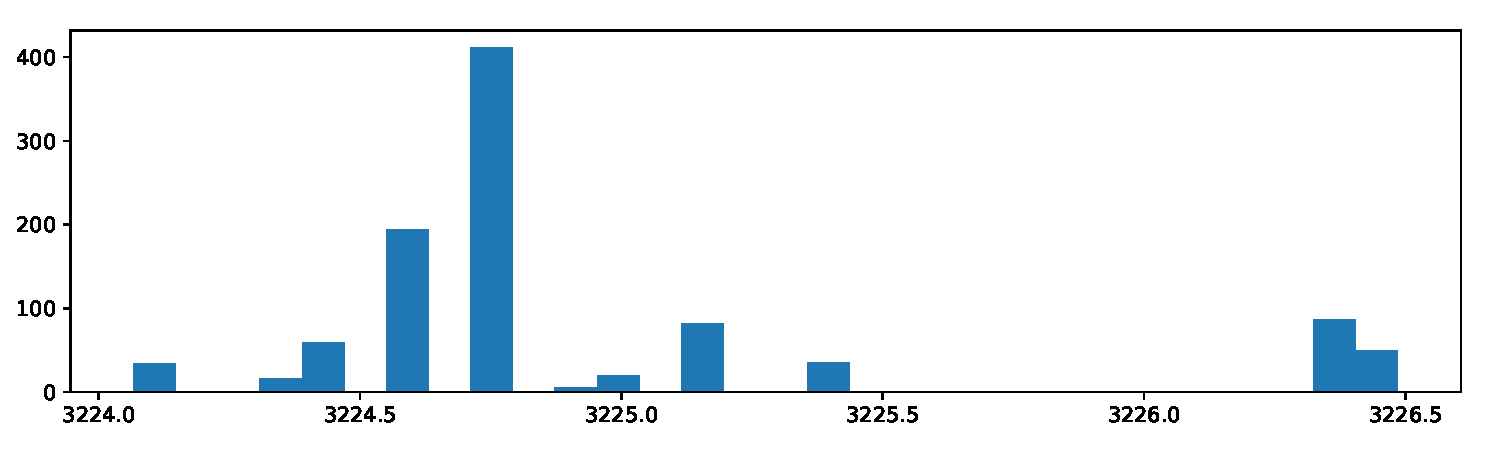
\includegraphics[width=0.7\linewidth]{Distortions.pdf}
 \caption{Histogram of distortions for 1000 random initializations of the K-means algorithm}
\end{figure}
\vfill

\textbf{3.b.} When we write $\Sigma_{j, t} = \sigma_{j, t} I$, the part of the likelihood to be maximized that depends on $\sigma$ is written
\begin{align*}
\sum_{i=1}^n \sum_{j=1}^k \tau_i^j\left(-\frac{n}{2}\log(\sigma_{j, t}) - \frac{1}{2\sigma_{j,t}} ||x_i - \mu_{j, t}||^2\right)
\end{align*}
For each j, the expression above is equal to $-\frac{n}{2}\log(\sigma_{j,t})\sum_i \tau_i^j - \frac{1}{2\sigma_{j,t}}\sum_i \tau_i^j ||x_i - \mu_{j,t}||^2$. They can be minimized separately. The gradient of this expression with respect to $\sigma_{j}$ reads: 
\begin{align*}
-\frac{n}{2\sigma_{j}}\sum_i \tau_i^j + \frac{1}{2\sigma_{j}^2} \sum_i\tau_i^j ||x_i - \mu_{j}||^2 = 0 \implies \boxed{\sigma_{j, t+1} = \frac{\sum_i\tau_i^j ||x_i - \mu_{j, t+1}||^2}{n \sum_i \tau_i^j}}
\end{align*}
The other derivations ($\mu$ and $\pi$) are the same than for the complete Gaussian mixture model detailed in the course notes.
\vfill

\textbf{3.c.} From the course notes we have $\boxed{\Sigma_{j,t+1} = \dfrac{\sum_i\tau_i^j(x_i-\mu_{j,t+1})(x_i-\mu_{j,t+1})^T}{ \sum_i\tau_i^j}}$
\vfill

\textbf{3.d.} For the isotropic gaussian model, the log-likelihood on the train set is -2649.9 and -2639 for the test set. Visually, the results for clustering are close to the results of K-means, which can be understood by the fact that the distance function used in K-means is the isotropic norm L2. However, the ``equivalent'' distance function in the isotropic Gaussian mixture model is non quadratic and therefore penalizes differently points far from a cluster center depending on the covariance of the cluster. 

The mixture of full gaussians allows for dealing with much more complex dataset shapes, which in the case of this dataset yields higher log-likelihoods: -2340.2 for the training set and -2431 for the test set. Estimations more closely ressemble the training data and are more accurate than the isotropic model as the test results show.
\vfill
 \clearpage
 \begin{figure}[t!]
\centering
\begin{subfigure}{.49\textwidth}
  \centering
  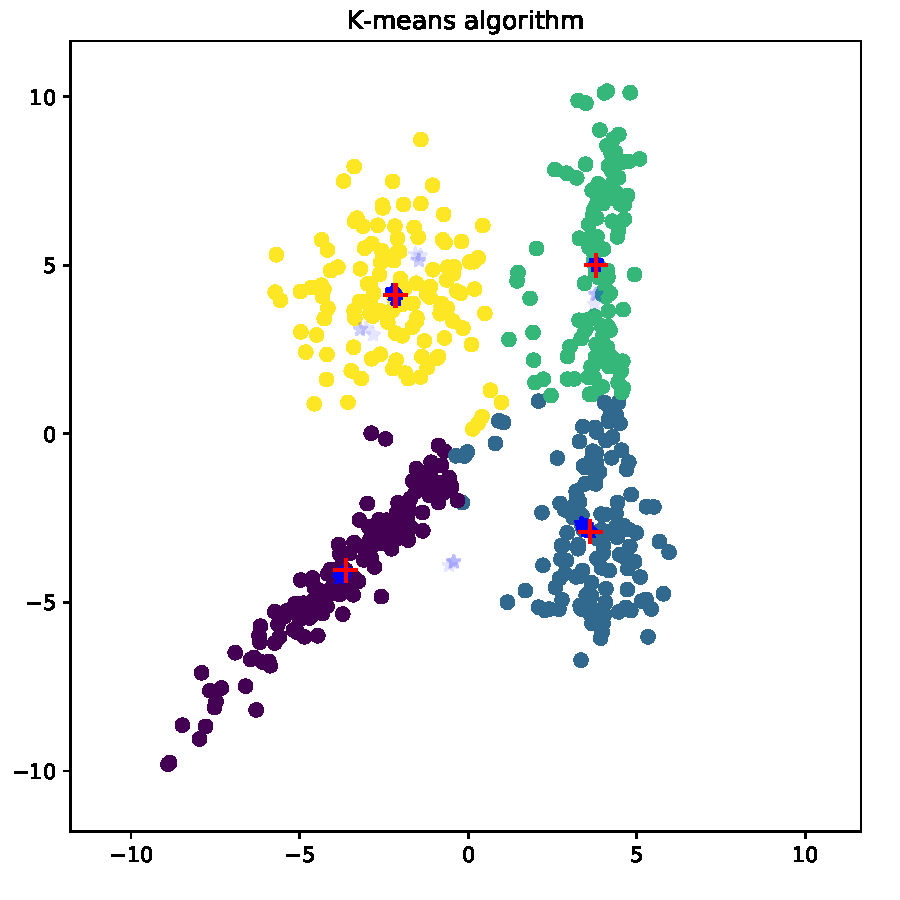
\includegraphics[width=\linewidth]{KMeans.pdf}

\end{subfigure} 
\begin{subfigure}{.49\textwidth}
  \centering
  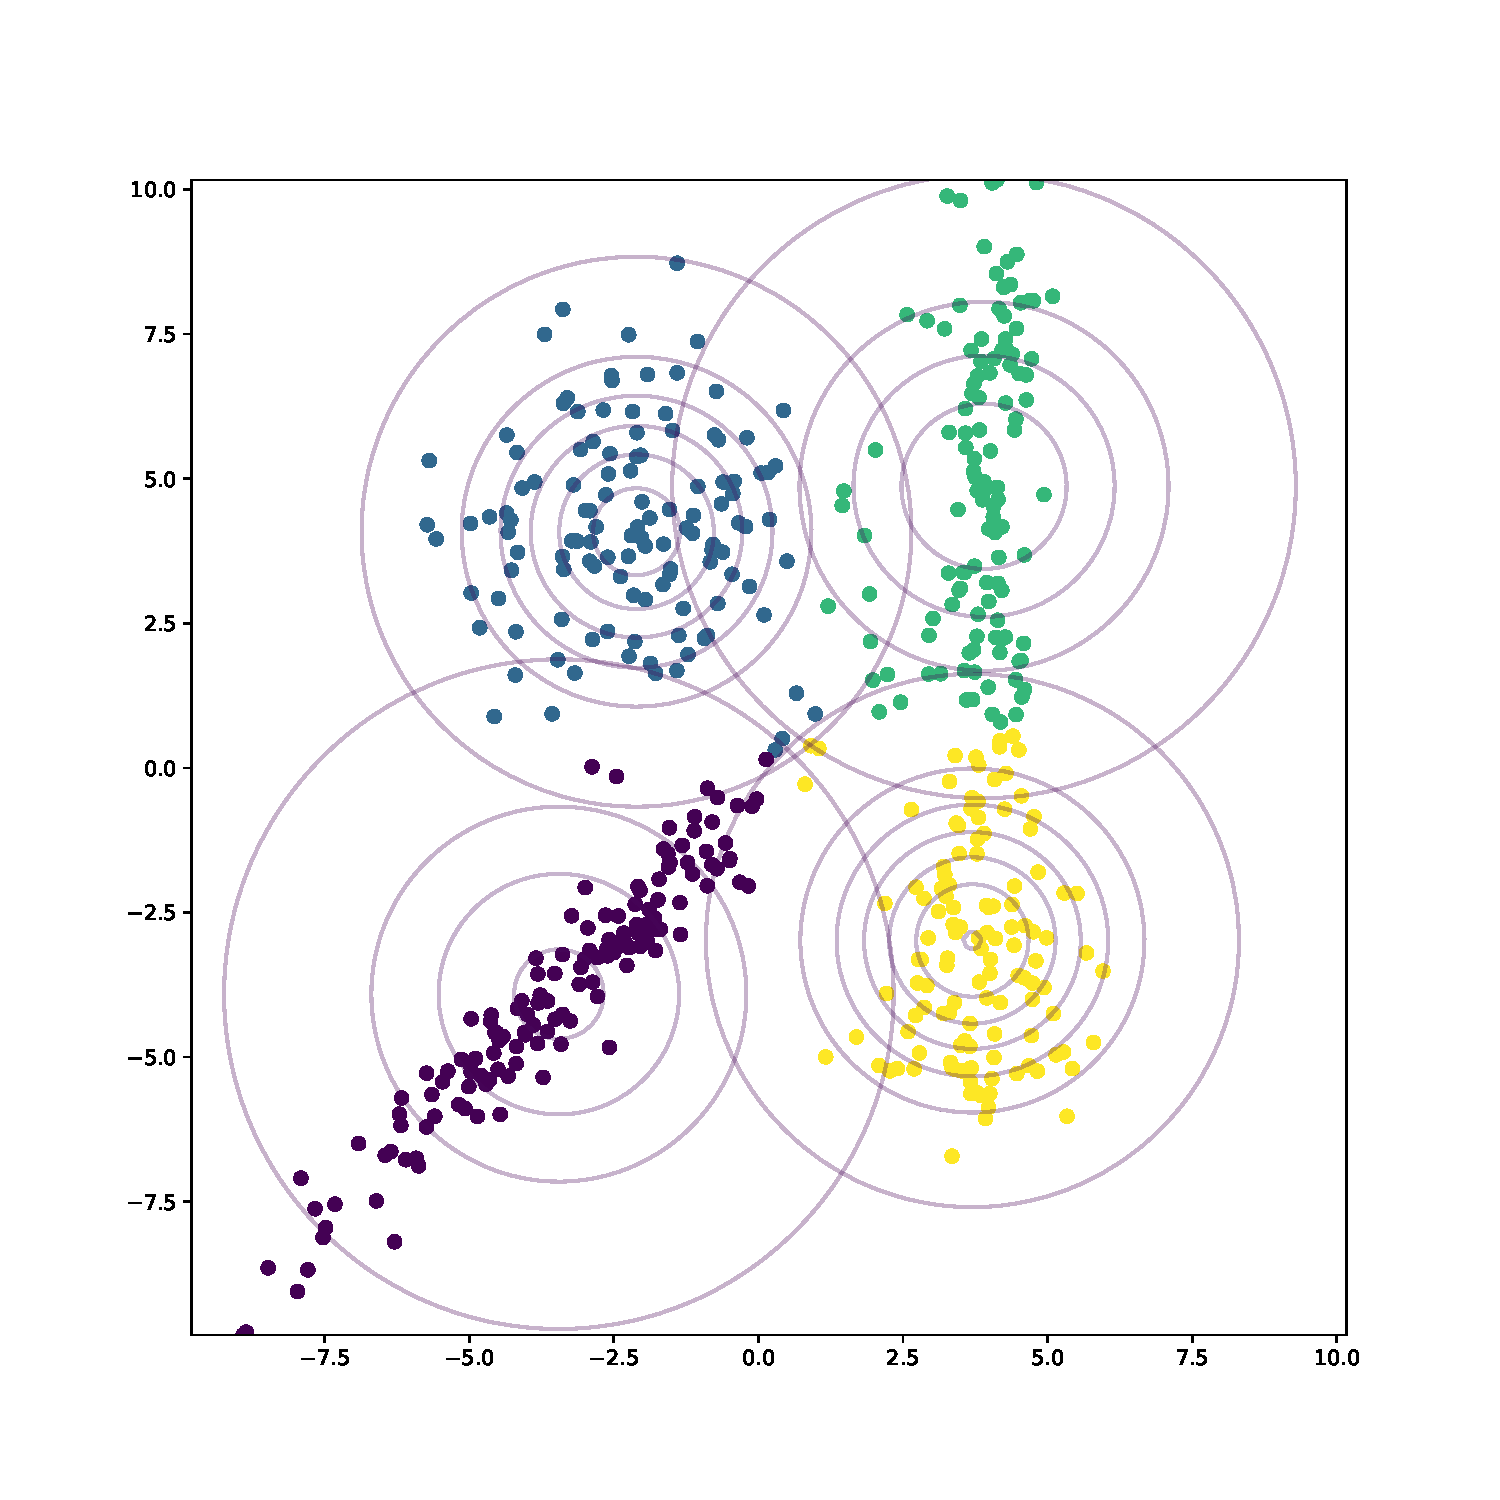
\includegraphics[width=\linewidth]{Isotropic.pdf}

\end{subfigure}
\\[+5pt]
\begin{subfigure}{.49\textwidth}
  \centering
  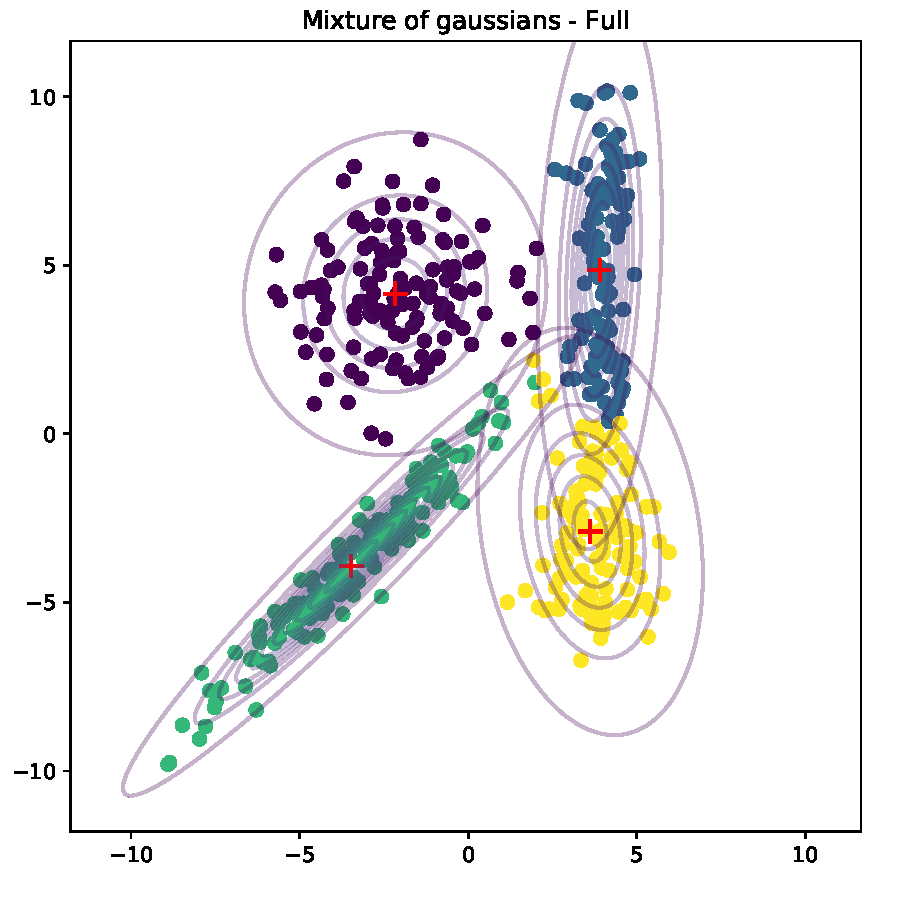
\includegraphics[width=\linewidth]{Full.pdf}

\end{subfigure} 

\end{figure}
 
 \end{document}